\chapter{Tagging Flavour at ATLAS}
\section{Introduction}
A fundamental ingredient in any ATLAS analysis is the ability to correctly identify particles in the aftermath of a collision, from $\tau$-leptons, to $b$- and $c$-quarks, and gluons $g$. Having well-calibrated and optimally performing b- and c-tagging tools is of primary importance in studies of the Higgs boson couplings to $b$- and $c$-quarks. It is also critical for top $t$-quark measurements and searches for extensions of the \gls{sm}. As described by the theory of \gls{qcd}, colour-charged objects, such as a $b$- or a $c$-quark, undergo hadronisation to form collections of colourless hadrons. These hadrons, mostly $B$ for $b$-quark and $D$ for $c$-quark, are unstable and further decay in the volume of the detector. Such a succession of decays leaves a collection of particles within a cone oriented in the direction of the original parton, an easily recognisable pattern referred to as a \textit{jet}. From an analysis of the complicated structure of the jet, the flavour of the initially decaying particle can be reconstructed. This is the task of \textit{flavour tagging}. In the ATLAS experiment, the tool to achieve this identification, called \textit{tagger}, is developed and maintained centrally by the \gls{ftag}. \\

Tagging $b$-jets benefits from a particularly advantageous configuration:  the $b$ is the lightest element of the third generation and must decay through a flavour-changing process. Because of the \gls{sm} all value of the $V_{bc}$ \gls{ckm} matrix element, this decay process is suppressed, giving $B$-hadrons a characteristically long-lifetime and decay length $(c\tau)_{B} \sim 400$  $\mu$m \cite{Tanabashi:2018oca}. When considering boosted objects with a Lorentz $\gamma$ factor above unity, the location of the $B$-hadron decay, called  \gls{sv}, can be reconstructed by the ATLAS pixel detector \cite{Aad:2019aic}. Other important variables describing the decay of $B$-hadrons are the \glspl{ip} $d_0$ and $z_0$ of charged particles emanating from the \gls{sv}. As shown in Figure \ref{fig:bjet}, $d_0$ and $z_0$ are the transversal and longitudinal distances from the primary vertex to the perigee\footnote{The point of closest approach.} of the track associated with the charged particle. For a $b$-jet, either or both of the \glspl{ip} can be large thanks to the long lifetime of the associated hadron. Other characteristics of $b$-jets are the large number of particles in the final state following their hadronisation, a property described as \textit{high multiplicity} which is due to the large mass of the $b$-quark, and the likely presence of leptons in the jet cone, as 40\% of the decays of $B$-hadrons including either an $e$ or a $\mu$ \cite{Tanabashi:2018oca}. \\

\begin{figure}[h!]
\center
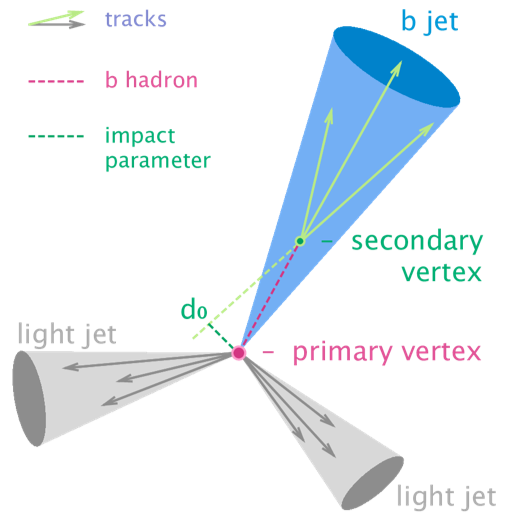
\includegraphics[scale=0.6]{Images/bjet}
\caption{Representation of a $b$-jet.} 
\label{fig:bjet}
\end{figure}

On the contrary, tagging $c$-jets, being at an intermediate scale between light- ($u$, $d$, $s$, and gluons) and $b$-jets, is much more challenging. The decay length for charged (neutral) $D$-hadrons, $(c\tau)_D \sim 300$ $(100)$ $\mu$m \cite{Tanabashi:2018oca}, is smaller than for $B$-hadrons and is difficult to resolve with the currently deployed tracker. The decay chain of $B$-hadrons often includes $D$-hadrons, making a clean separation of $c$-jets from $b$-jets harder. Compared to $b$-jets, $c$-jets have a lower multiplicity which leads to $\tau$-jets being easily mistaken for $c$-jets, as these leptons can hadronically decay into a sufficiently large number of particles to mimic a jet in the detector. For all these reasons, less effort has been historically dedicated to constructing $c$-taggers in ATLAS. The task is however gaining particular attention due to the focus on the challenging $H \rightarrow c\bar{c}$ search \cite{Aaboud:2018fhh}. This chapter presents the development of a novel $b$- and $c$-tagger for the ATLAS experiment. \\

\section{Flavour Tagging at ATLAS}

In the ATLAS experiment, a choice was made to develop centrally a tagger to be used by the whole collaboration. It relies on a dedicated set of algorithms to perform simultaneously $b$- and $c$-tagging and is continuously improved to meet the requirements of the physics program. Currently, all adopted approaches rely on \gls{dl} methods, given their vastly superior effectiveness. These \gls{dl} methods rely on high-level features reconstructed by sub-algorithms based on physics variables, such as the tracks \glspl{ip}, and the reconstruction of secondary vertices. The low-level algorithms consist of \cite{Paganini:2289214}:
\begin{itemize}
\item Jet Fitter: a vertexing algorithm based on a Kalman filter to reconstruct the topology and fit the decay chain \gls{pv} $\rightarrow$ $B$ $\rightarrow$ $D$ with the assumption that the vertices of the weakly decaying B/D-hadrons tend to align with the \gls{pv} \cite{ATL-PHYS-PUB-2018-025}. 
\item \gls{sv1}: combining a secondary vertex finder and a tagger to offer flavour discrimination information. The former, based on the VKalVrt vertex reconstruction package \cite{Kostyukhin:685551}, returns a list of candidate secondary vertices with measured quantities assigned to each vertex. The latter derives jet weights based on discriminative variables and computes properties of the \gls{sv}, such as the mass. 
\item \gls{ip} likelihood: IP2D and IP3D are both likelihood-based methods to assign flavour-discriminating weights based, respectively, on the transversal and global impact parameters significance (corresponding to the reweighted \gls{ip} variables by their respective uncertainties) of the tracks \cite{ATLAS:2017bcq}. 
\item Track collection analyser: either with \gls{rnnip} \cite{ATL-PHYS-PUB-2017-003} or \gls{dips} \cite{ATL-PHYS-PUB-2020-014}. These are \textit{Neural Network} (NN) approaches to extract discrimination information on the set of tracks associated with a jet. These taggers are further described later in this section.  
\end{itemize}

\begin{figure}[h!]
\centerline{
\begin{minipage}[c]{0.4\textwidth}
    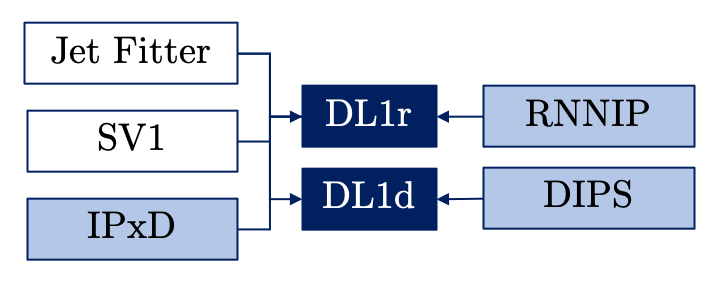
\includegraphics[scale=0.5]{Images/Algorithms}
  \end{minipage}
\begin{minipage}[c]{0.6\textwidth}
    \caption{The algorithms for flavour tagging at ATLAS. High-level taggers are in dark blue, track-based taggers in light blue and vertex-related taggers in white.}
    \label{fig:algo}
  \end{minipage}
 }
  \end{figure}

The outputs of these low-level algorithms, as well as certain jet-related variables, such as $p_T$, are then combined as input to a high-level tagger consisting of a fully-connected \gls{nn} called \gls{dl1r} or \gls{dl1d}, respectively if \gls{rnnip} or \gls{dips} is used. The input vector is typically made of 44-45 features. This high-level tagger outputs three probabilities $p_X$ for the analysed jet to correspond to a $b$-, $c$-, or light--flavour (indicated with the letter $u$) such that $p_b + p_c + p_u = 1$. A $b$-tagging score $D_b$ is then derived by computing a scaled log-likelihood ratio: 
\begin{equation}\label{bdisc}
D_b = \log \frac{p_b}{f^b_c \times p_c + (1 - f^b_c) \times p_u},
\end{equation}
where $f^b_c$ is the charm fraction, a parameter that can be modified to tweak the importance of each flavour. The analogous $c$-tagging score $D_c$ is: 
\begin{equation}\label{cdisc}
D_c = \log \frac{p_c}{f^c_b \times p_b + (1 - f^c_b) \times p_u}.
\end{equation}

A jet is $X$-tagged if the $D_X$ discriminant score is above a set threshold constant $c_{wp}$, defining a \textit{Working Point} (WP) with a unique configuration of signal and background (mis-tag) efficiencies. In this context, the efficiency $\epsilon^X_Y$ for $Y$-flavour jets to be $X$-tagged and the corresponding rejection $\mathcal{R}^X_Y$ are respectively defined as:
\begin{equation}
\epsilon^X_Y = \frac{N^{X-tagged}_{Y-jets}}{N_{Y-jets}} \quad \textrm{and} \quad \mathcal{R}^X_Y = \frac{1}{\epsilon^X_Y},
\end{equation}
where $N^{X-tagged}_{Y-jets}$ and $N_{Y-jets}$ are respectively the number of $X$-tagged $Y$-flavoured jets and the total number of $Y$-flavoured jets. \\

These high-level models are trained on \gls{mc} simulated data samples and need to be calibrated on real data to deliver an unbiased estimate, by deriving \glspl{sf} weights correcting the predictions for each jet. Uncertainties are derived on the predicted score and passed along to analyses using the tool. The novel algorithm introduced in this work is the \gls{dl1d} tagger, which relies on the \gls{dips} sub-tagger to extract correlations between the tracks.  

\subsection{RNNIP}
The \gls{rnnip} tagger runs on arbitrary-length input sequences made of track features, as ordered by the absolute transverse \gls{ip} significance, to extract tagging information from correlations between tracks \cite{ATL-PHYS-PUB-2017-003}. The vector of track features includes the transverse and longitudinal impact parameter significances, the jet $p_T$ fraction carried by the track, the distance between the track and the jet axis, and a learned 2D embedding of the track quality \cite{Paganini:2289214}. It outputs a probability $p_X$ for the jet to belong to flavour $X$ $\in$ [$b$, $c$, light].

\subsection{DIPS}
The \gls{dips} tagger, based on the Deep Sets architecture \cite{NIPS2017_f22e4747}, is a \gls{gnn} approach to model the correlations between an arbitrary number of tracks. Two NNs are trained in this effort. A model $\Phi$ maps each individual track feature vector (similar to \gls{rnnip}) to a latent space (forming the nodes of the graph). The representations of each track in this latent space are then concatenated by a simple summation operation (the edges of the graph) and given as input to a secondary \gls{nn} model $F$ outputting the predicted probability $p_X$ for the jet to belong to flavour $X$ $\in$ [$b$, $c$, light] (the prediction of the graph). This approach has several advantages over \gls{rnnip}, mainly the physically motivated permutation-invariance of the input and the improved training/evaluation time thanks to a more parallelisable architecture. Furthermore, the performance delivered by \gls{dips} is observed to globally outperform \gls{rnnip} \cite{ATL-PHYS-PUB-2020-014}. 

\section{Samples and Training Procedure}
In preparation for the next run of the LHC, ATLAS has improved its reconstruction software. As such, important aspects of flavour tagging have changed, requiring to retrain the taggers to ensure optimal performance. This work presents the first ATLAS study of the retraining of \gls{dl1r} on the new release (R22) and the inclusion of \gls{dips} in the complete flavour tagging tools, a tagger called \gls{dl1d}. Another novelty is the possible inclusion of $\tau$-jets, to improve their rejection from c-jets. However, due to the widespread use of the FTAG algorithms and the difficulties arising in calibrating a tagger with exceptionally good rejection against $\tau$-jets, these are not included in the default version of the tagger nor in the results shown here.  \\ 

Two samples from proton-proton collisions at $\sqrt{s} = 13$ are simulated for this analysis:
\begin{itemize}
\item $t\bar{t}$ events, with at least one of the $W$-boson from the top-quark decay further decaying leptonically. 
\item $Z'$ events, where an exotic boson $Z'$ decays as $Z' \rightarrow q\bar{q} \textrm{ or } \tau \bar{\tau}$, with a variable $Z'$ mass to generate a flat $p_T$ spectrum extending the $p_T$-range of the jets studied up to 4 TeV.
\end{itemize}

For both samples, the ATLAS detector is simulated using GEANT4 \cite{Agostinelli:602040} and jets are reconstructed with the anti-kT algorithm with a radius of R = 0.4.  For \gls{rnnip}, the tracks considered must pass the following quality selection: $\geq$ 7 hits in the silicon layers, $\leq$ 2 missing hits in the silicon layers, $\geq$ 1 hit in the pixel detector, $\leq$ 1 hit shared by multiple tracks, $p_T$ > 1 GeV, $|d_0|$ < 1 mm, and $|z_0 \textrm{ sin}(\theta)|$ < 1.5 mm. For \gls{dips}, a looser track selection is applied to capture more tracks, modifying the nominal selection in the following way: $p_T$ > 0.5 GeV, $|d_0|$ < 3.5 mm, and $|z_0 \textrm{ sin}(\theta)|$ < 5 mm \cite{ATL-PHYS-PUB-2020-014}. Loosening the selection was observed to lead to a significant improvement in performance for jets with a $p_T < 250$ GeV for \gls{dips}. \\

These two samples are combined into a hybrid sample to train the taggers, with 70\% of the total number of jets coming from $t\bar{t}$ and the remaining from the $Z'$. The $t\bar{t}$ and $Z'$ samples cover, respectively, a low- and high-$p_T$ region based on a reconstructed $B$-hadron $p_T$ separation threshold of 250 GeV for $b$-jets and a jet $p_T$ of 250 GeV for non-$b$-jets. The evaluation of the performance of a trained tagger is performed on the separated sets and unfolded over the flavours.\\

ATLAS flavour tagging tools are widely used across the collaboration. It is therefore important for the taggers not to learn specific features of the simulations used for training but to focus on the inherent differences between the studied flavours. The hybrid sample is therefore downsampled in [$p_T - \eta$] bins to have the same number of $b$-, $c$-, and light-jets in each 2D bin. The total statistics available is of $25 \times 10^{6}$ jets per flavour for training. The $t\bar{t}$ and $Z'$ samples for validation and testing are each made of 1 million jets and are not downsampled.\\

Training is done with the Umami framework \cite{Umami} based on TensorFlow \cite{tensorflow2015-whitepaper} for 300 epochs with a variable learning rate schedule and the default network structure adopted in already released \gls{dl1r}: 8 fully connected \gls{nn} of smoothly-decreasing sizes in [256, 128, 60, 48, 36, 24, 12, 6] with ReLu activation leading to a final softmax layer producing the predicted probabilities for each flavour. While the \gls{dips} probabilities used as inputs to \gls{dl1d} come from a model trained on the new release, the \gls{rnnip} probabilities are still from a model trained on the previous one (R21) \cite{ATL-PHYS-PUB-2017-003, ATL-PHYS-PUB-2020-014}. Indeed, due to the large difference in performance, \gls{rnnip} is no longer supported in the new release and is included for sake of comparability to the previous techniques. The models at an epoch offering the best combined results in terms of $b$-tagging efficiency and rejection from $b$-jets on the validation set are selected for further analysis. Importantly, every training converged to a fixed set of performance values, with no overtraining occurring.\\

Several modifications to the model architecture, list of input variables, and preprocessing and training procedures have been explored, with no significant gain observed:
\begin{itemize}
\item The preprocessing steps were revised to reduce the size of the evaluation sets for the benefit of the training one. A dual approach, down-sampling light-jets and up-sampling $c$-jets to the $b$-jets [$p_T - \eta$], has also been implemented. This approach uses importance sampling with replacement to obtain the same fraction of the different flavours and the same $p_T$ and $|\eta|$ distribution. While the performance of the majority classes was observed to improve, the efficiency at tagging the upsampled minority class ($c$-jets) was slightly lower. This trade-off can be controlled by modifying the flavour fractions. 
\item Several modifications to the list of input features have been attempted, with no clear advantage uncovered. Adding pile-up information (the actual number of interactions per crossing and the number of primary vertices were tested) was not observed to have an impact on the tagging efficiency. Adding other variables from \gls{sv1} or JetFitter was also not observed to improve performance. However, a positive observation is that the IP2D and IP3D taggers can both be safely removed without change to performance, as the information they add is in all likelihood now covered by the \gls{dips} sub-tagger, thereby reducing the list of sub-taggers to maintain.
\item The structure of the network and its training procedure. Using samples produced with an older release of the ATLAS software to pre-train the model was not observed to deliver a boost in performance. Changing the size of the network and the batch size was also not observed to have a positive effect.
\end{itemize}

The performance of the retrained \gls{dl1r} tagger on the new release was found to be in good agreement with the currently recommended \gls{dl1r}, despite using the same training of \gls{rnnip} on the previous release.  

\section{Analysis of Results}
In order to establish a meaningful benchmark for the newly trained taggers, the performance of the recommended \gls{dl1r} tagger, trained and evaluated on an analogous set of samples from the previous release, is included in the following results as benchmark under the label \textit{Recom. \gls{dl1r} }. \\

Figure \ref{fig:DL1dtt} presents the \gls{roc} curves on the $t\bar{t}$ (left) and $Z'$ (right) samples for  $b$-tagging. These \gls{roc} plots show, on the $x$-axis, the $b$-tagging efficiency ($\epsilon^b_b$ ) versus, on the $y$-axis, the rejection $\mathcal{R}^b_Y$ for $Y \in$ [$c$, light]. The two bottom sub-plots present the ratio of the c-jet rejection and light-jet rejection curves to the blue ones. This blue curve is the recommended \gls{dl1r} performance and serves as the baseline of the comparison, while the new tagger \gls{dl1d} is plotted in orange. Figure \ref{fig:DL1dz} shows the same plots for $c$-tagging, with respect to $b$- and light-jet rejection.  The important observation is the clear gain obtained when replacing \gls{rnnip} with \gls{dips}. Both the $b$- and $c$-tagging performance of \gls{dl1d} clearly dominate the \gls{dl1r} version, with a significant improvement in background flavour rejection for all tagging efficiency considered, as summarised in Table \ref{tab:max-perf}. The largest improvement in performance is obtained for $b$-tagging on the $t\bar{t}$ process, corresponding to a lower jet momentum. \\

In the light-rejection from $b$-jets \gls{roc} curves in Figure \ref{fig:DL1dtt}, there is an elbow in the curve at high $b$-jet efficiency. This effect is also present in the $b$-rejection from $c$-tagging, in Figure \ref{fig:DL1dz}. Both correspond to a set of, respectively, light-jets and $b$-jets that do not overlap with the $b$-jets $b$-tagging and $c$-jets $c$-tagging discriminants distributions, as shown in Figures \ref{fig:scoreDL1dtt} and \ref{fig:scoreDL1dz}. These ``background`` jets are easily removed from the core set of ``signal'' jets due to internal differences between the flavours and the discrete nature of some sub-taggers used.  \\

The background rejections of the various taggers for $b$-tagging ($c$-tagging) as a function of the jet transverse momentum at a fixed $b$-efficiency of 70\% ($c$-efficiency of 30\%) per region displayed are shown in Figure \ref{fig:ptDL1dtt} (Figure \ref{fig:ptDL1dz}). Throughout the $p_T$ range considered, \gls{dl1d} outperforms the \gls{dl1r} tagger. The low $p_T$ $b$-rejection from $c$-jets is noticeably better for the retrained tagger compared to \gls{dl1r}. 

%
\begin{center}
\vspace{-1.cm}
\begin{figure}[h!]
\centerline{
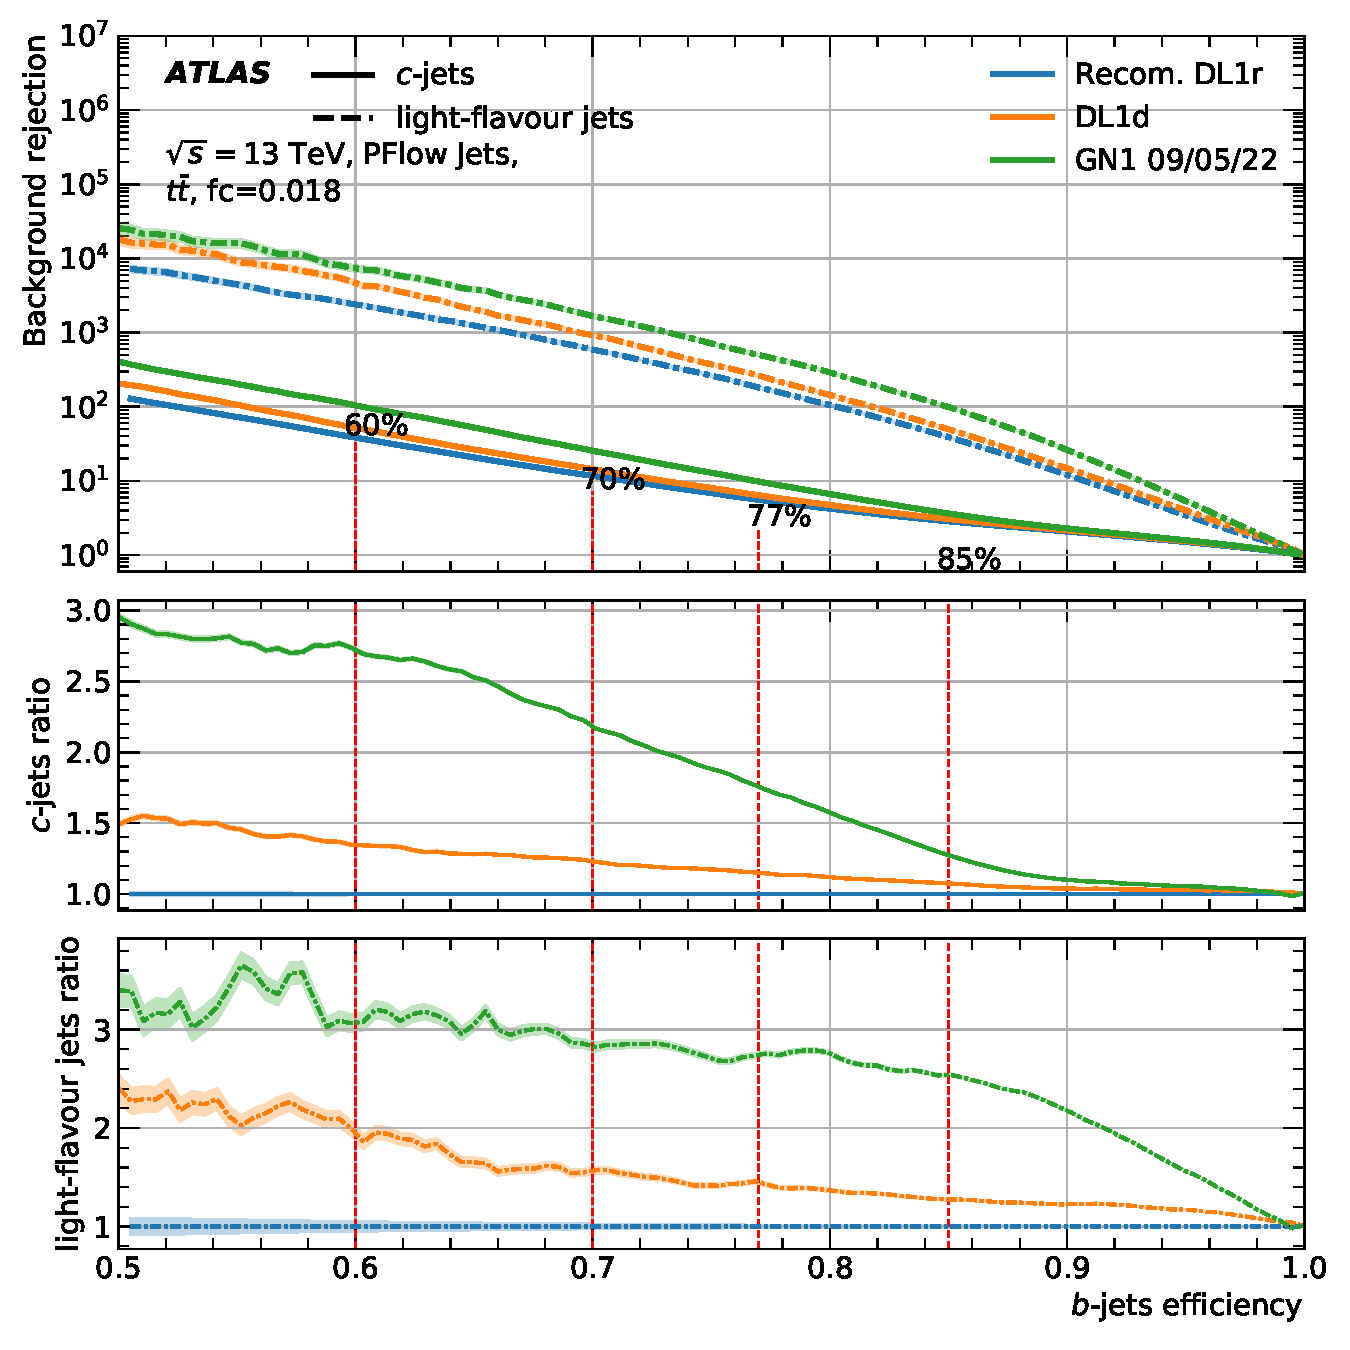
\includegraphics[scale=0.45]{Images//FTAG/Reprocessed/plotting_alone/ttbar_comparisons_300.pdf}
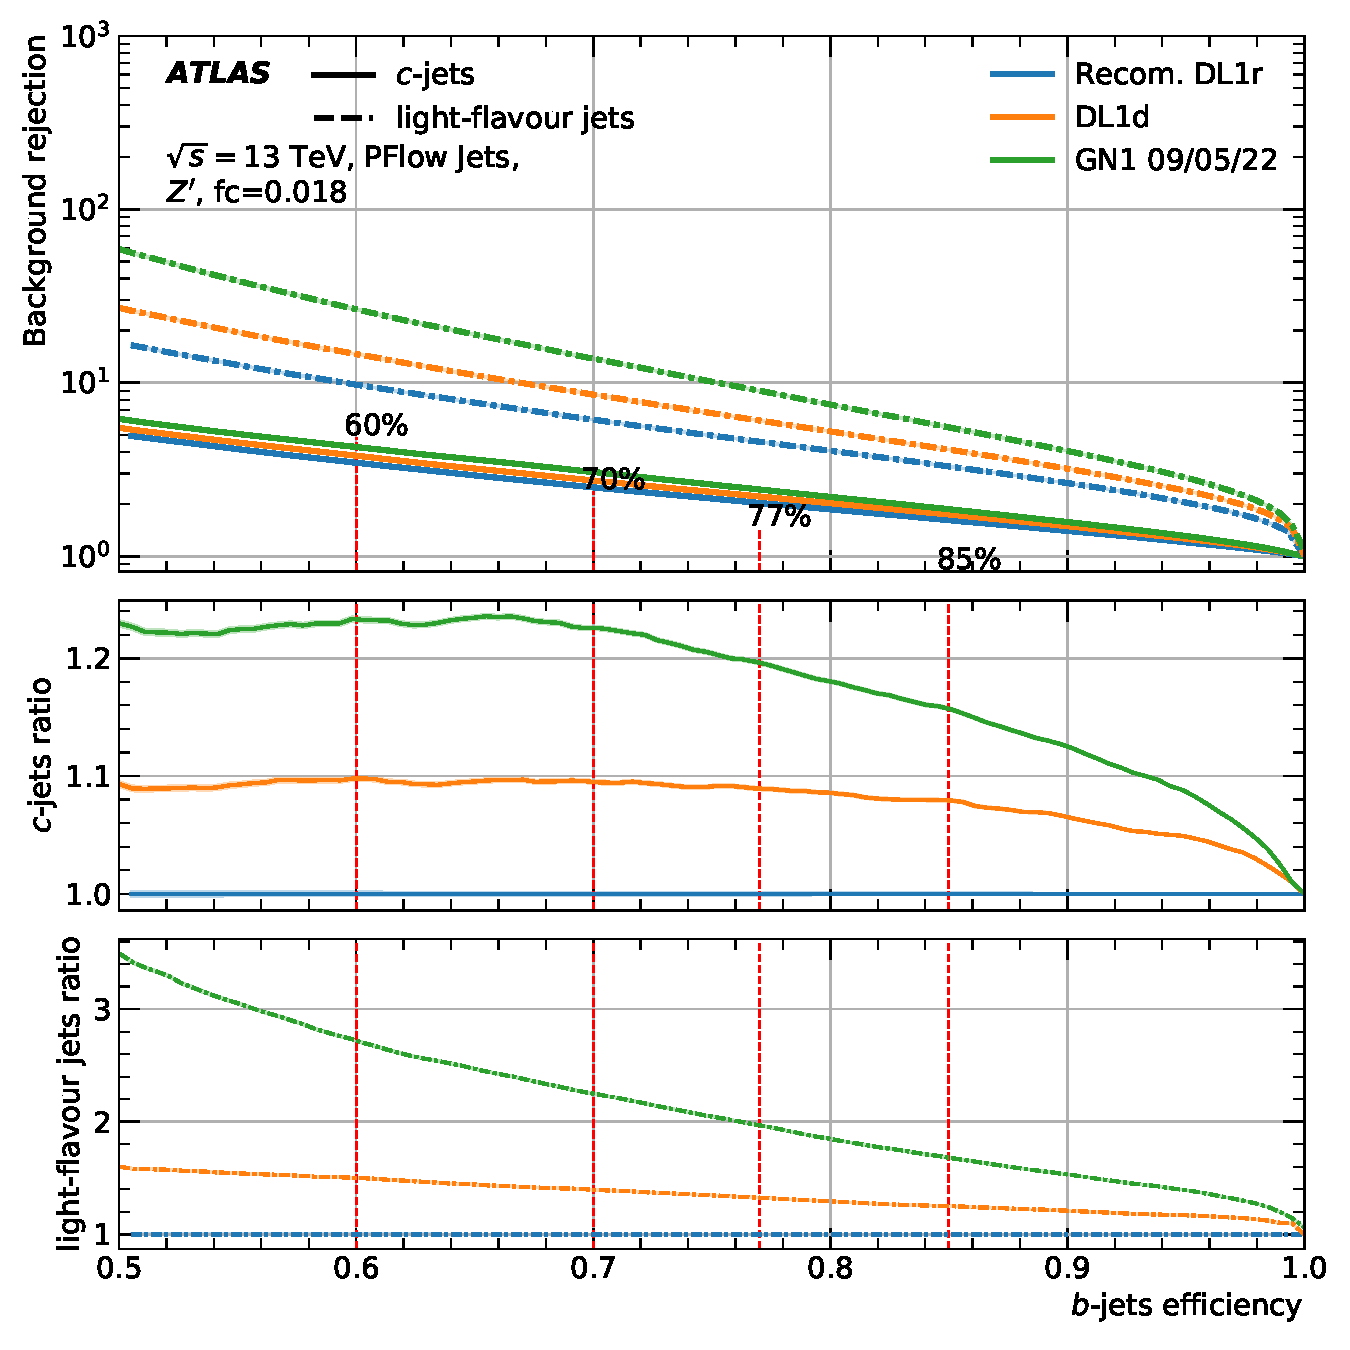
\includegraphics[scale=0.45]{Images//FTAG/Reprocessed/plotting_alone/zp_comparisons_300.pdf}
}
\caption{Performance for $b$-tagging with a flavour fraction of $f^b_c = 0.018$. Left: $t\bar{t}$; right: $Z'$. Top: \gls{roc} curves; centre: ratio of $c$-jets rejection from $b$-jets relative to the R22-retrained \gls{dl1r}; bottom: same ratio for light-jets rejection. List of taggers: {\color{blue} recommended \gls{dl1r} from the previous release}; {\color{orange} \gls{dl1d} trained on the new release}; {\color{greenforest} \gls{gn1} test-model trained on the new release}.}
\label{fig:DL1dtt}
\bigskip
\centerline{
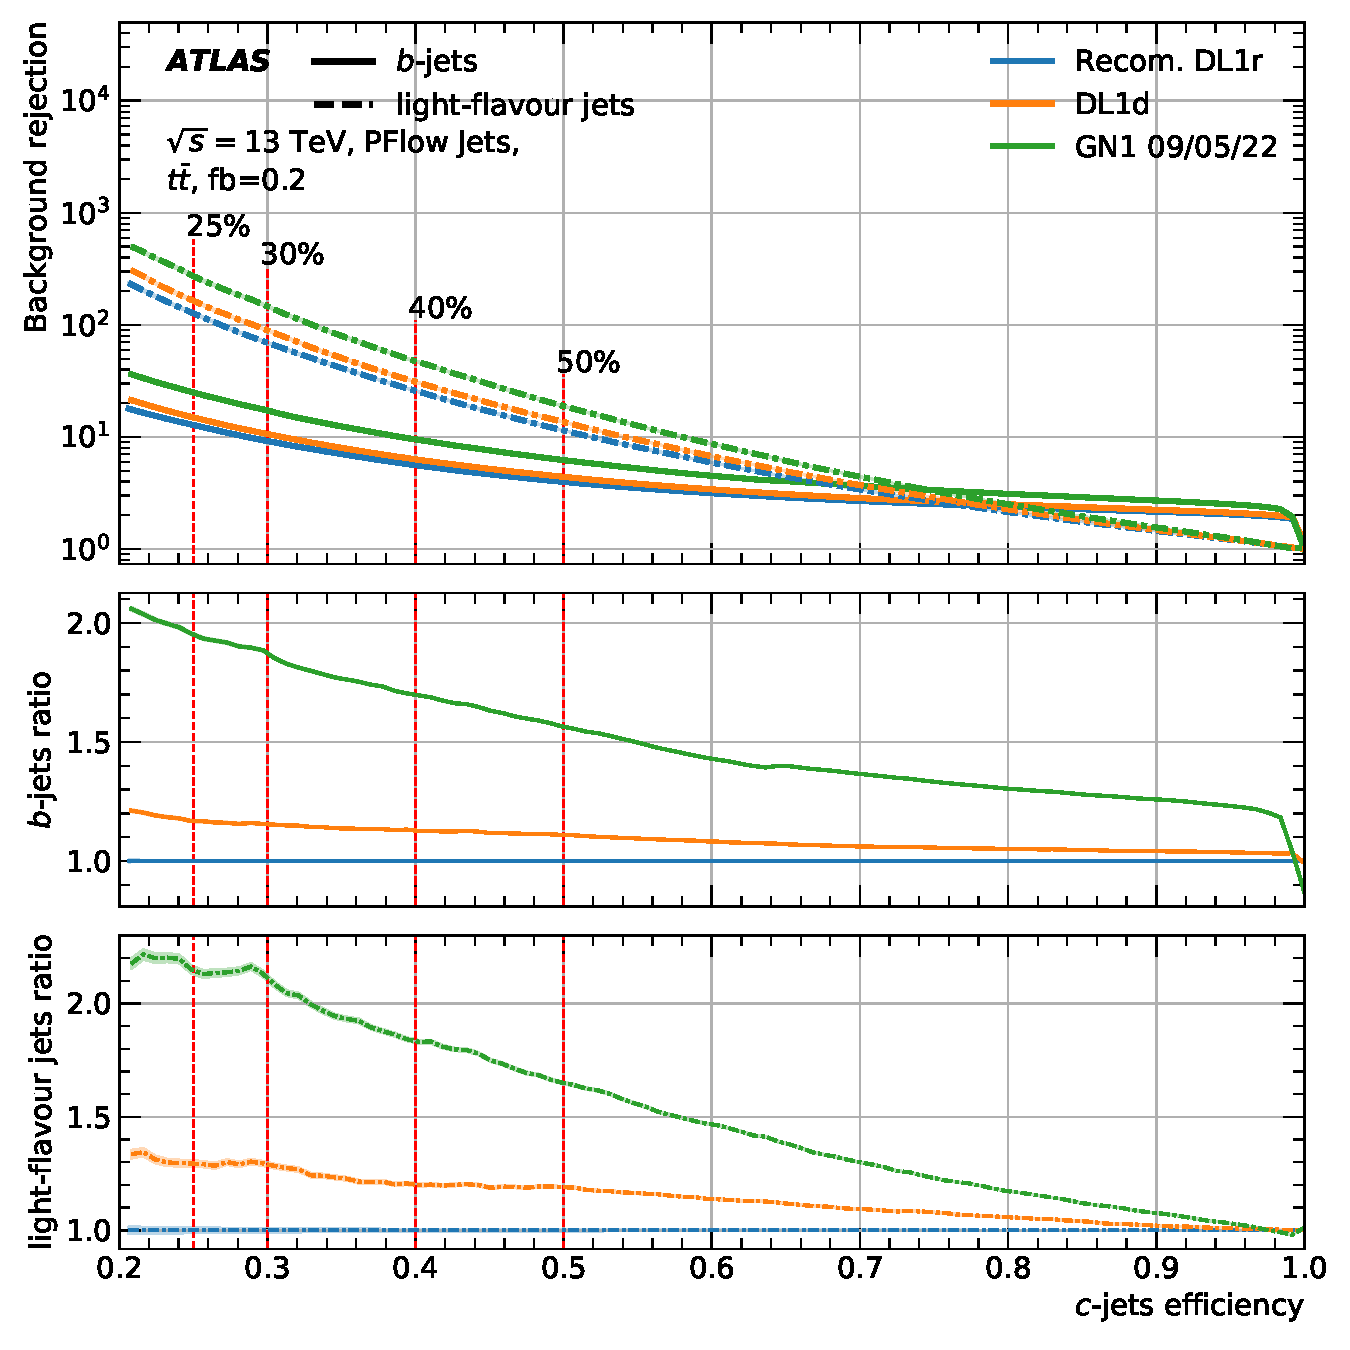
\includegraphics[scale=0.45]{Images/FTAG/Reprocessed/plotting_alone_c/ttbar_comparisons_299.pdf}
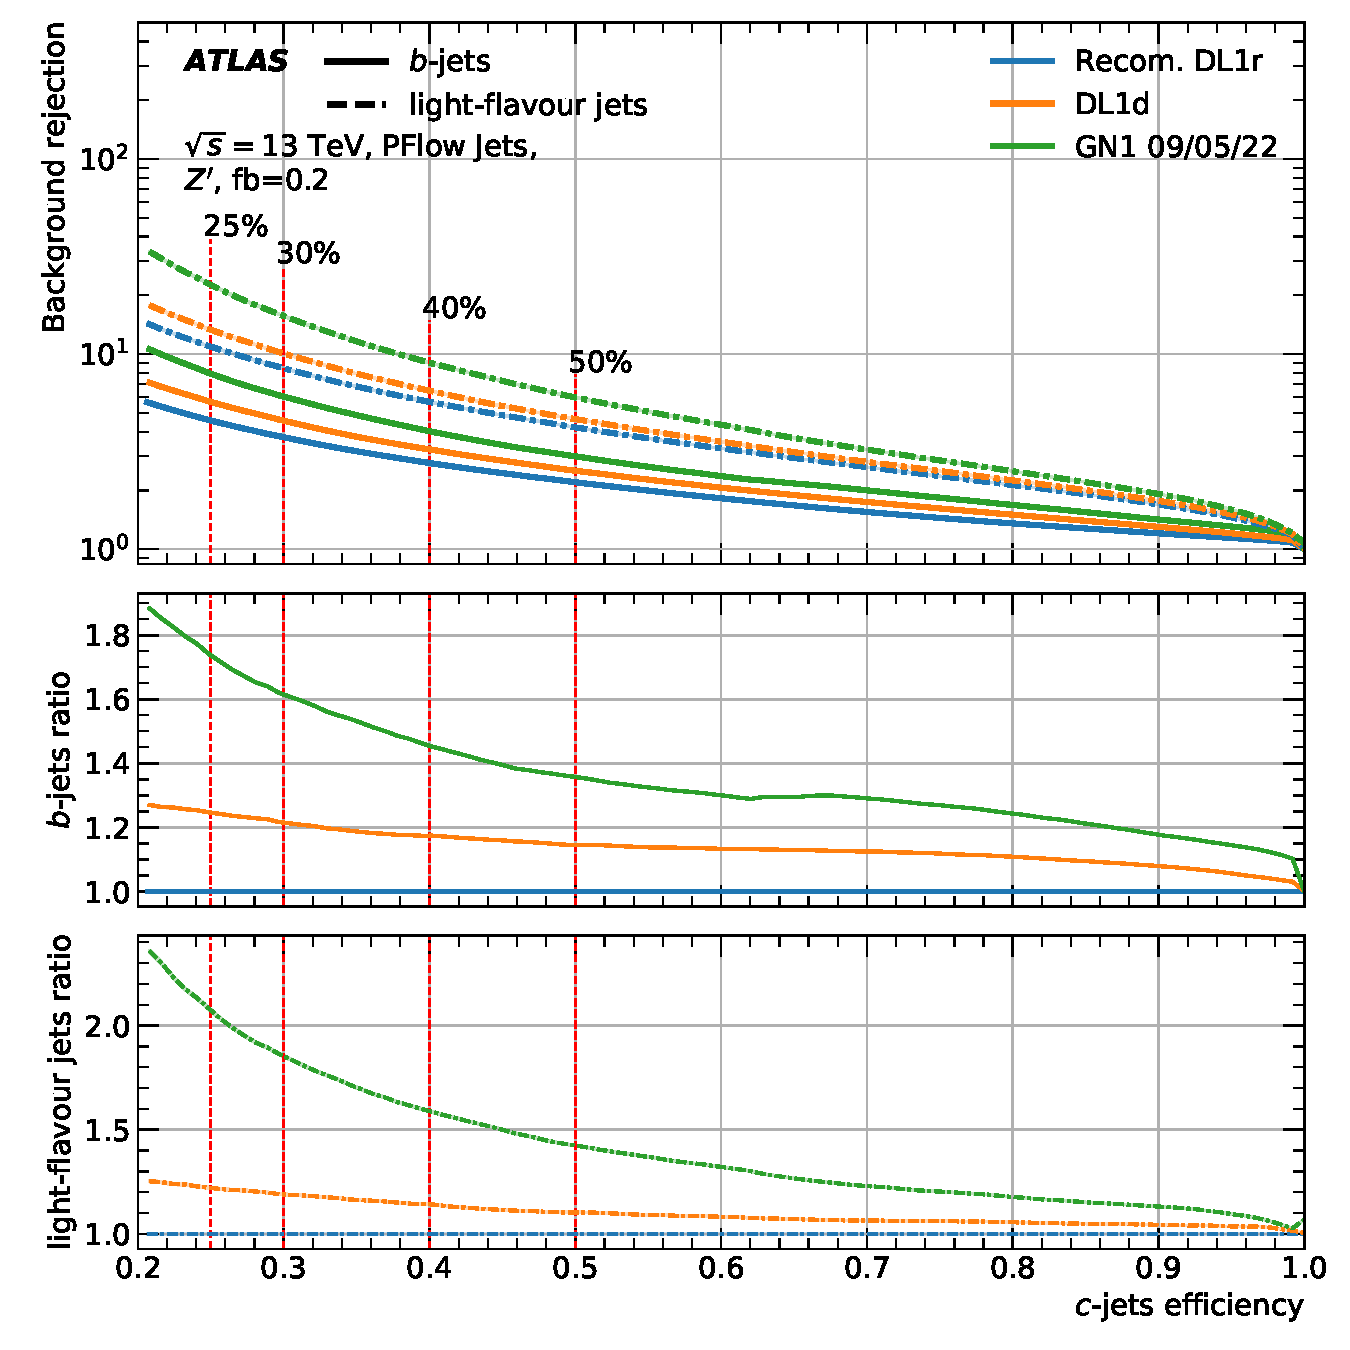
\includegraphics[scale=0.45]{Images/FTAG/Reprocessed/plotting_alone_c/zp_comparisons_299.pdf}
}
\caption{Performance for $c$-tagging with a flavour fraction of $f^c_b = 0.2$. Left: $t\bar{t}$; right: $Z'$. Top: \gls{roc} curves; centre: ratio of $b$-jets rejection from $c$-jets relative to the R22-retrained \gls{dl1r}; bottom: same ratio for light-jets rejection. List of taggers: {\color{blue} recommended \gls{dl1r} from the previous release}; {\color{orange} \gls{dl1d} trained on the new release}; {\color{greenforest} \gls{gn1} test-model trained on the new release}.}
\label{fig:DL1dz}
\end{figure}
\end{center}
%
\clearpage

\begin{table}[h]
  \begin{center}
      \begin{tabular}{C{2cm}|cc} 
      	 \hline \hline
          \multicolumn{3}{c}{$b$-tagging on $t\bar{t}$} \\ \hline
          WP & $c$-rejection  & light-rejection  \\ \hline
          60\%   & +26\% & +73\% \\ 
          70\%   & +19\% & +56\% \\ 
          77\%   & +12\% & +41\% \\ 
          85\%   & +7\%   & +32\% \\ \hline
          \multicolumn{3}{c}{} \\
           \hline  \hline
           \multicolumn{3}{c}{$c$-tagging on $t\bar{t}$} \\ \hline
          WP & $b$-rejection  & light-rejection  \\ \hline
          25\%   & +26\% & +5\% \\
          30\%   & +25\% & +9\% \\
          40\%   & +22\% & +12\% \\
          50\%   & +18\% & +15\% \\ \hline
      \end{tabular}
      \quad
       \begin{tabular}{C{2cm}|cc} 
       	 \hline  \hline
          \multicolumn{3}{c}{$b$-tagging on $Z'$} \\ \hline
          WP & $c$-rejection  & light-rejection  \\ \hline
          60\%   & +19\% & +43\% \\
          70\%   & +10\% & +32\% \\
          77\%   & +9\%  & +26\% \\
          85\%   & +6\%  & +19\% \\ \hline
          \multicolumn{3}{c}{} \\
           \hline  \hline
           \multicolumn{3}{c}{$c$-tagging on $Z'$} \\ \hline
          WP & $b$-rejection  & light-rejection  \\ \hline
          25\%   & +12\% & +22\% \\
          30\%   & +11\% & +19\% \\
          40\%   & +8\%   & +14\% \\
          50\%   & +7\%   & +10\% \\ \hline  \hline
      \end{tabular}
    \caption{The ratio of background flavour rejection of the \gls{dl1d} to \gls{dl1r} at various tagging efficiencies, both trained on the new release. Top: $b$-tagging ($f^b_c = 0.018$); bottom: $c$-tagging  ($f^c_b = 0.2$); left: $t\bar{t}$; right: $Z'$.}
    \label{tab:max-perf}
  \end{center}
\end{table}

%
\begin{center}
\begin{figure}[h!]
%\vspace{-0.2cm}
\centerline{
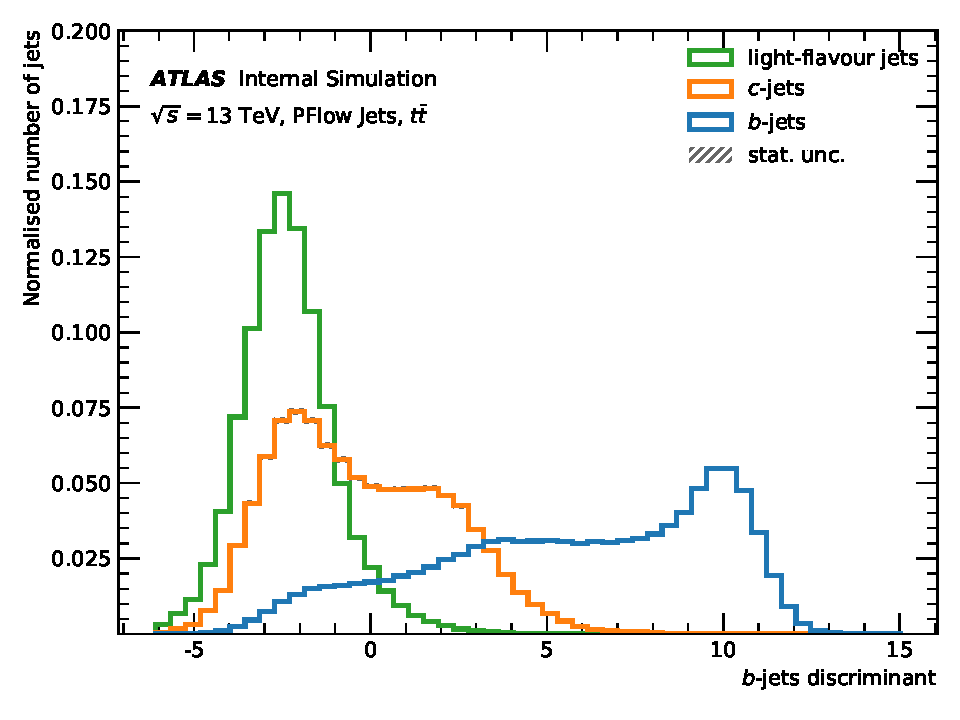
\includegraphics[scale=0.5]{Images//FTAG/Reprocessed/plotting_variables/scores_DL1_ttbar_300.pdf}
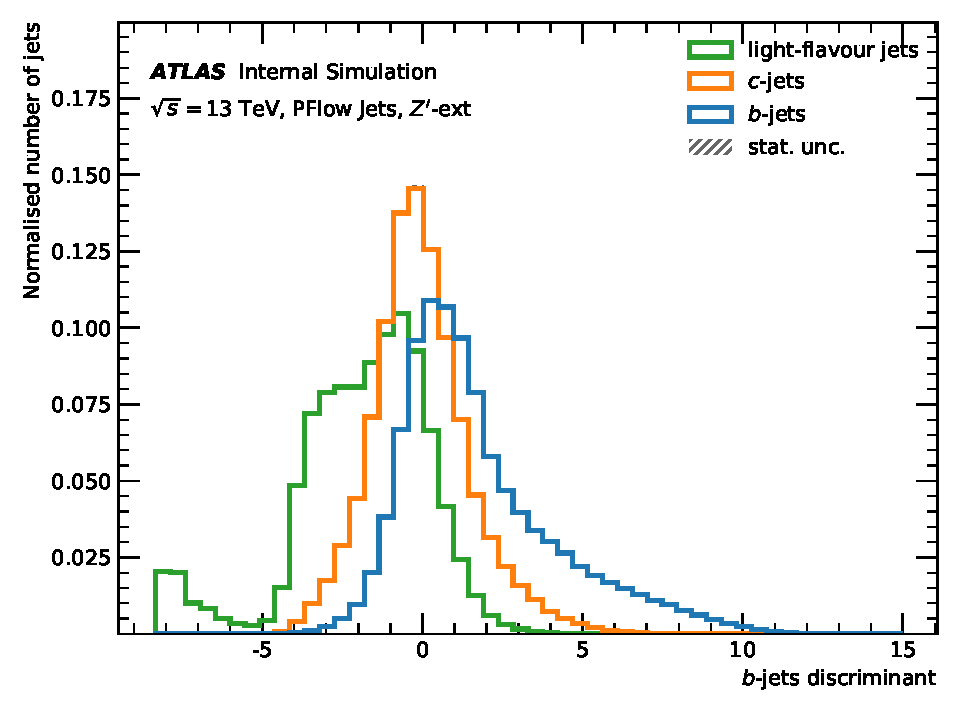
\includegraphics[scale=0.5]{Images//FTAG/Reprocessed/plotting_variables/scores_DL1_zprime_300.pdf}
}
\caption{Distribution of \gls{dl1d} $b$-tagging discriminant for the different jet flavours, evaluated on $t\bar{t}$ (left) and $Z'$ (right).}
\label{fig:scoreDL1dtt}
\centerline{
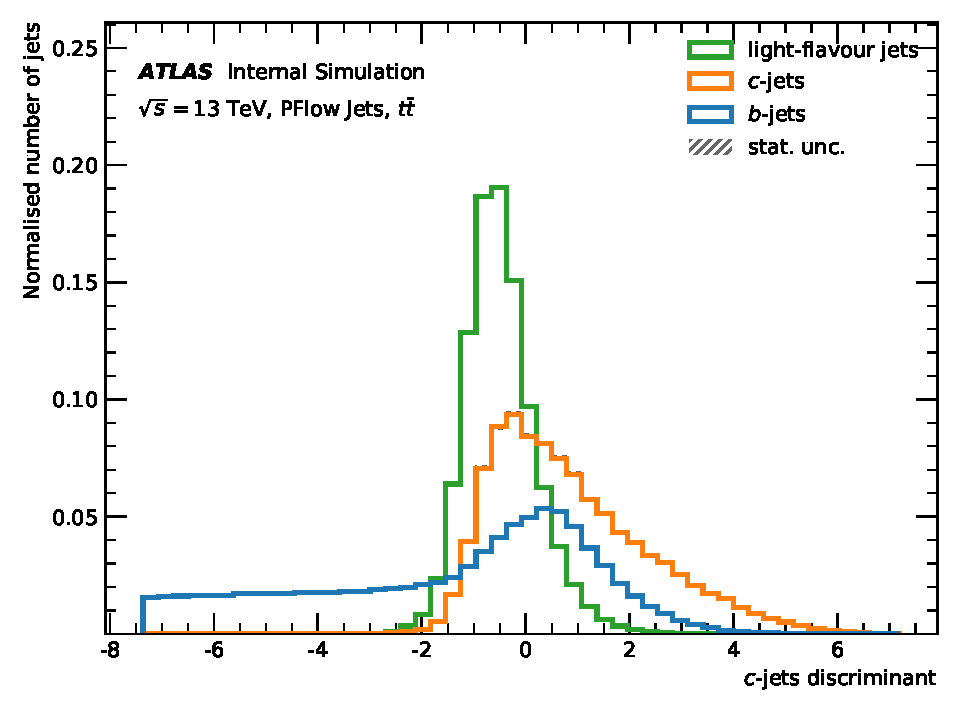
\includegraphics[scale=0.5]{Images/FTAG/Reprocessed/plotting_variables_c/scores_DL1_ttbar_c_299.pdf}
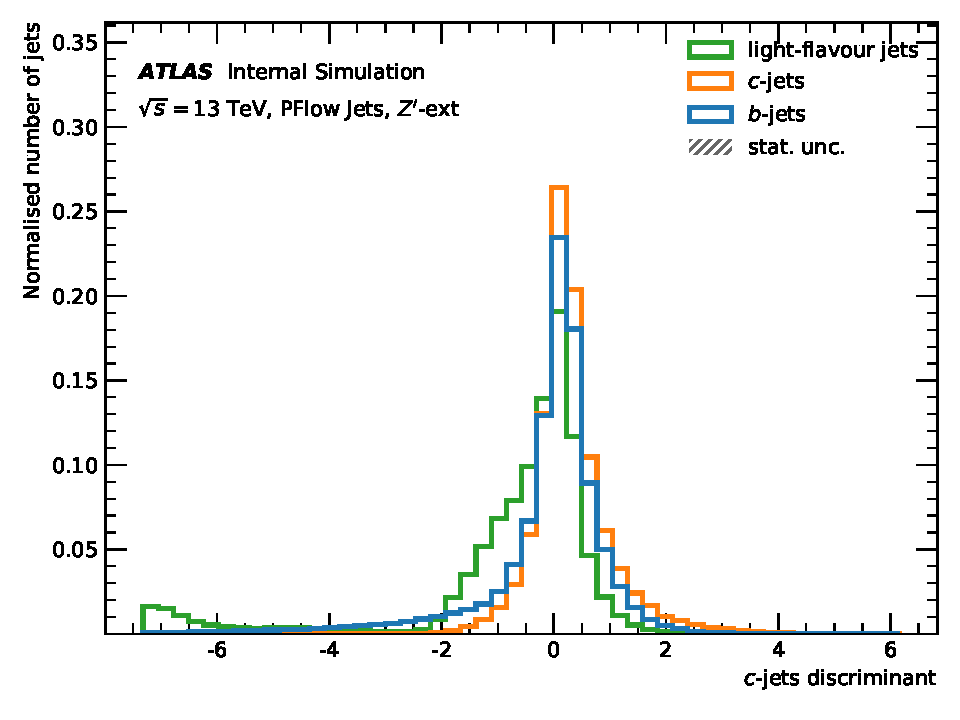
\includegraphics[scale=0.5]{Images/FTAG/Reprocessed/plotting_variables_c/scores_DL1_zprime_c_299.pdf}
}
%\vspace{-0.3cm}
\caption{Distribution of \gls{dl1d} $c$-tagging discriminant for the different jet flavours, evaluated on $t\bar{t}$ (left) and $Z'$ (right).}
\label{fig:scoreDL1dz}
\end{figure}
\end{center}
%

\clearpage
%
\begin{center}
\begin{figure}[h!]
\vspace{-0.55cm}
\centerline{
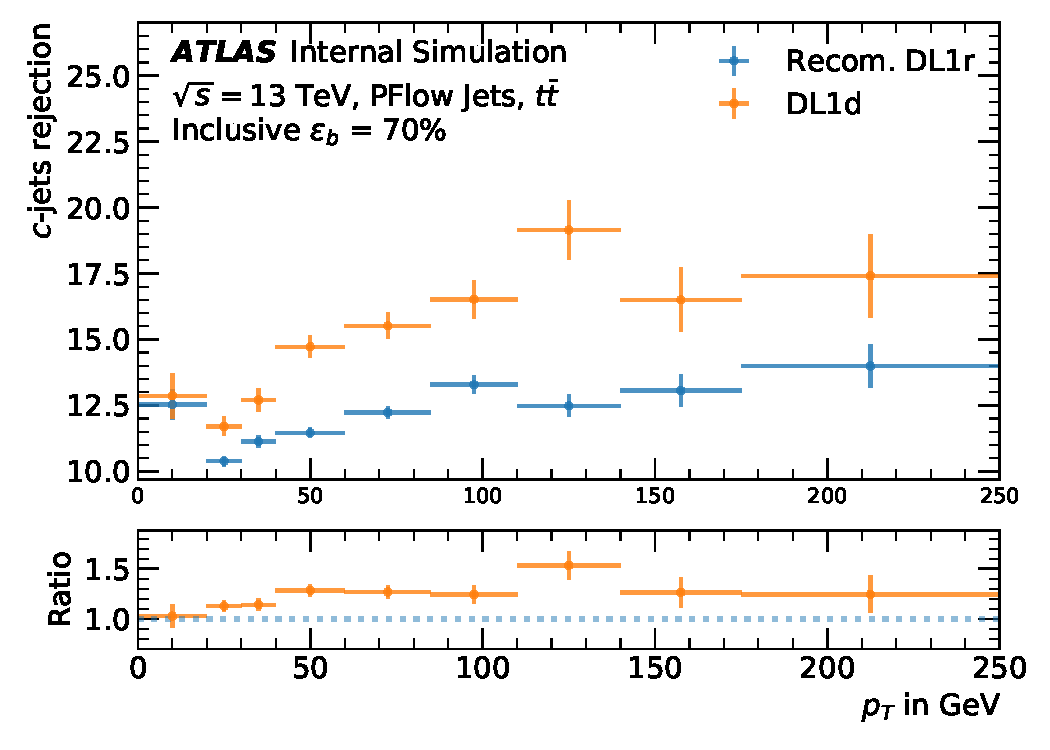
\includegraphics[scale=0.425]{Images//FTAG/Reprocessed/plotting_eff_vs_pt/pT_vs_beff_c_tt_300.pdf}
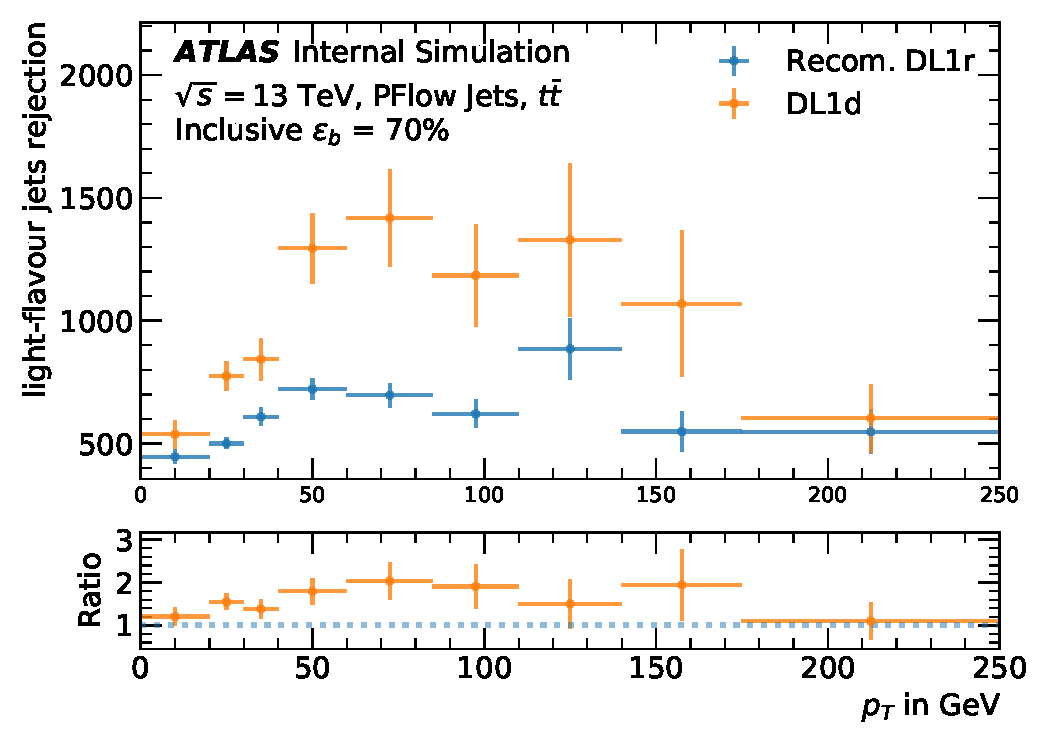
\includegraphics[scale=0.425]{Images//FTAG/Reprocessed/plotting_eff_vs_pt/pT_vs_beff_u_tt_300.pdf}}
\centerline{
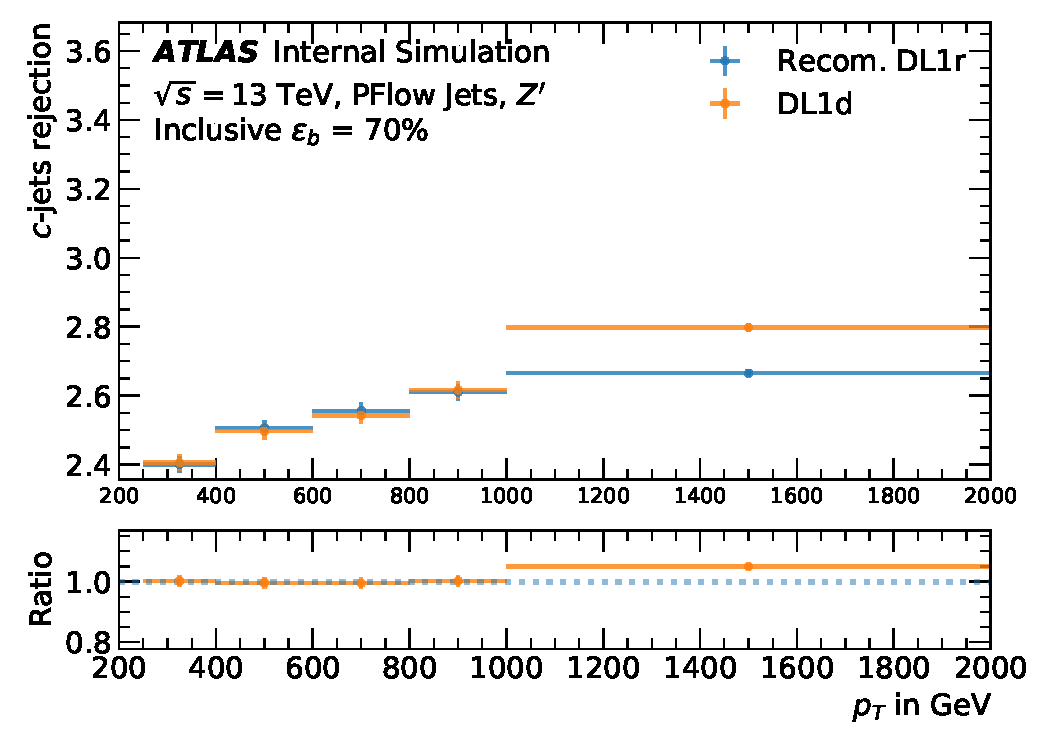
\includegraphics[scale=0.425]{Images//FTAG/Reprocessed/plotting_eff_vs_pt/pT_vs_beff_c_zp_300.pdf}
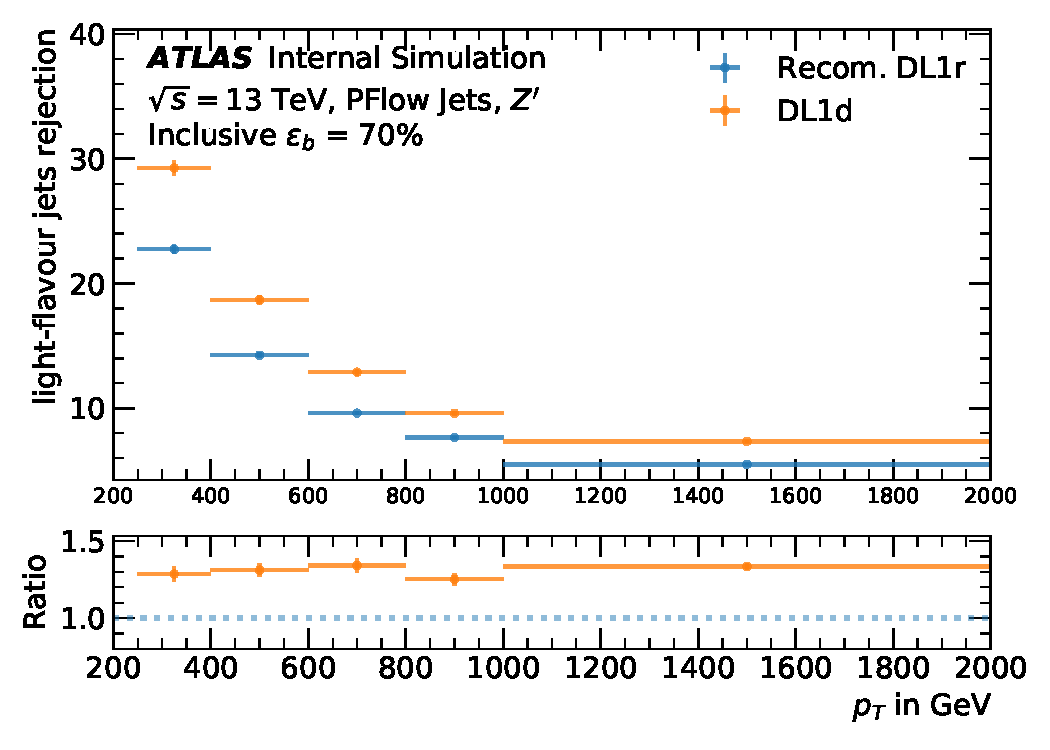
\includegraphics[scale=0.425]{Images//FTAG/Reprocessed/plotting_eff_vs_pt/pT_vs_beff_u_zp_300.pdf}
}
\caption{Background flavour rejections at a fixed $b$-tagging efficiency of 70\% (per region shown) for the various taggers. Top: $t\bar{t}$; bottom: $Z'$; left: $c$-rejection; right: light-rejection. For each plot, the bottom panel presents the ratio to the recommended \gls{dl1r}.}
\label{fig:ptDL1dtt}
\bigskip
\centerline{
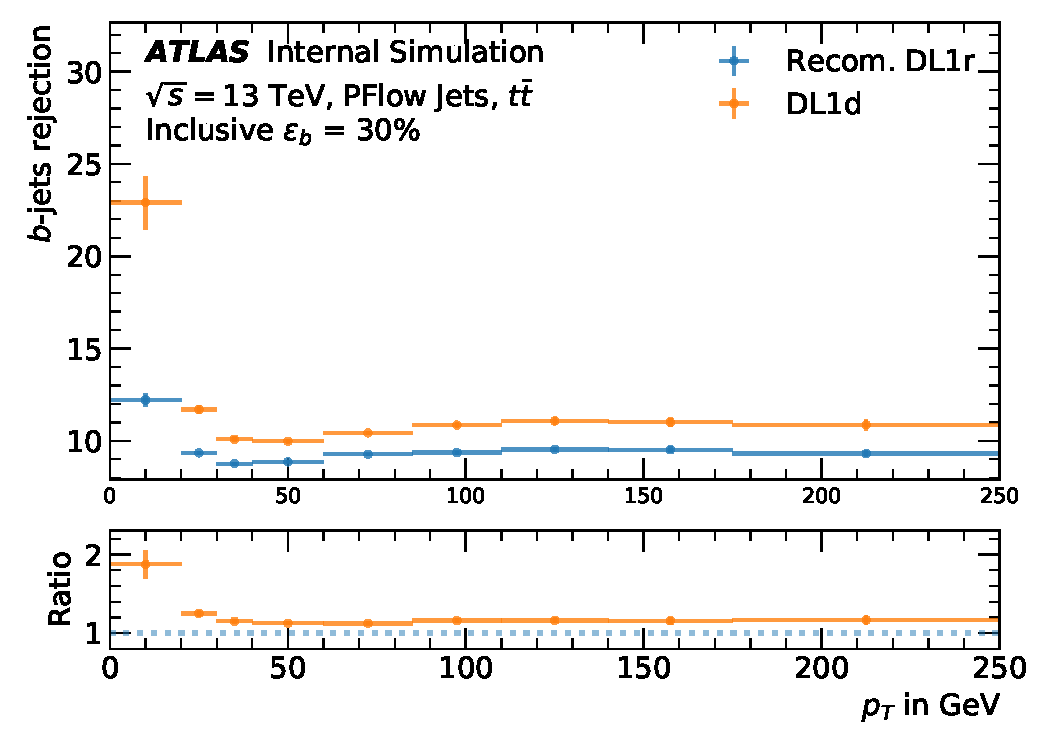
\includegraphics[scale=0.425]{Images//FTAG/Reprocessed/plotting_eff_vs_pt_c/pT_vs_beff_c_tt_299.pdf}
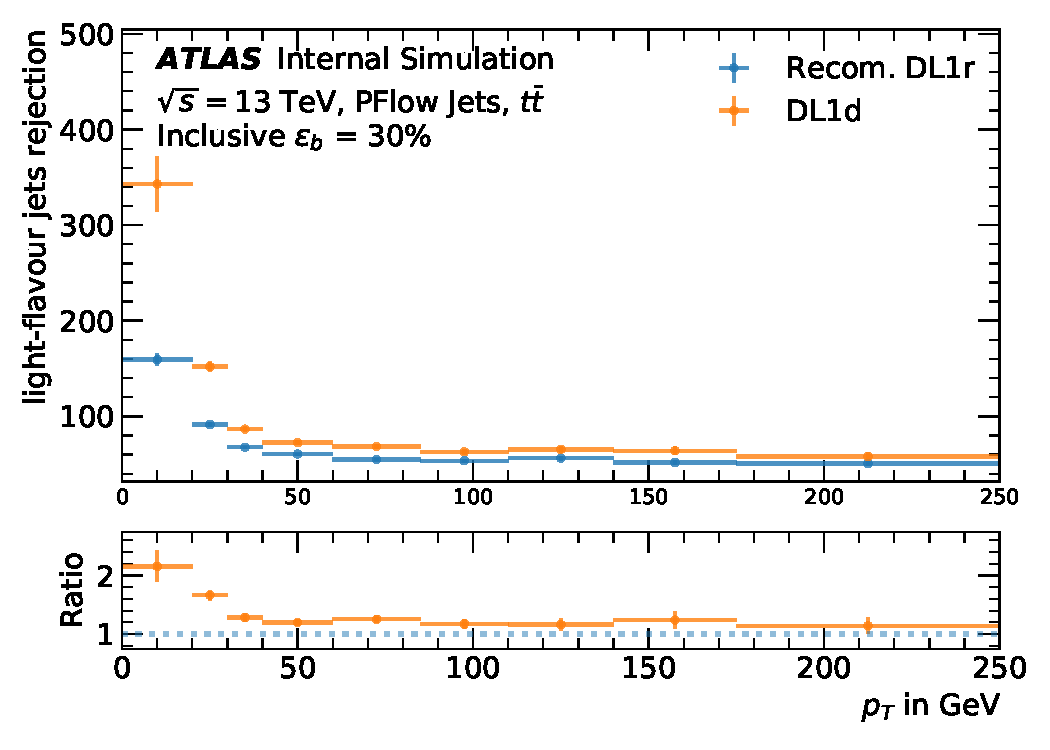
\includegraphics[scale=0.425]{Images//FTAG/Reprocessed/plotting_eff_vs_pt_c/pT_vs_beff_u_tt_299.pdf}}
\centerline{
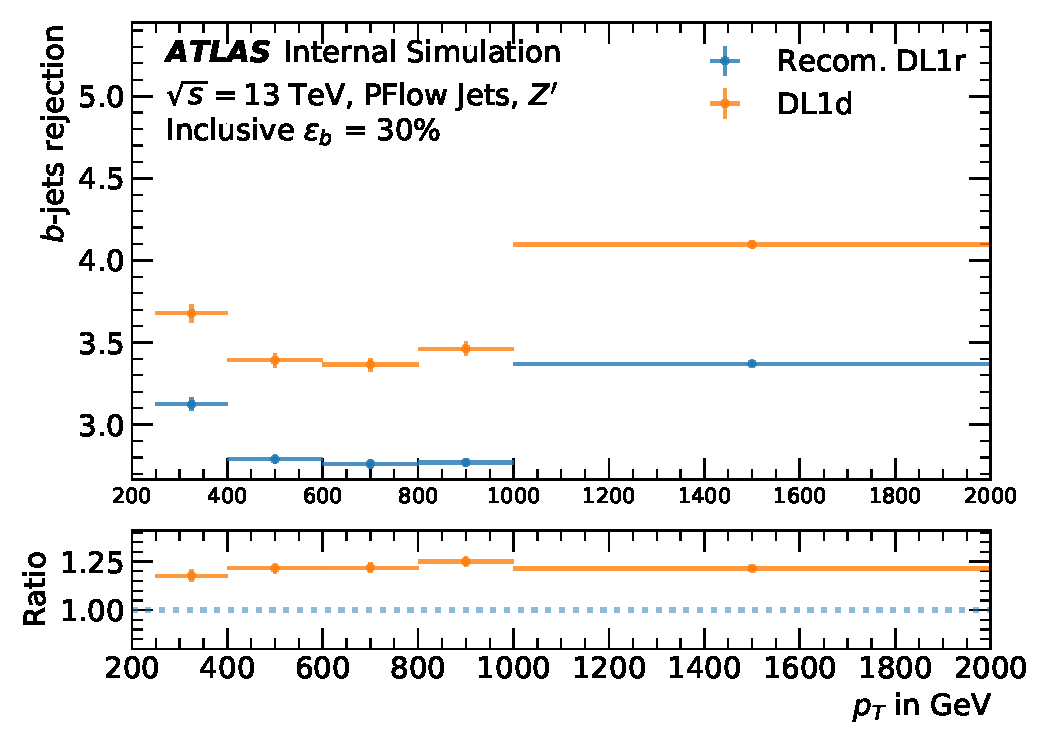
\includegraphics[scale=0.425]{Images//FTAG/Reprocessed/plotting_eff_vs_pt_c/pT_vs_beff_c_zp_299.pdf}
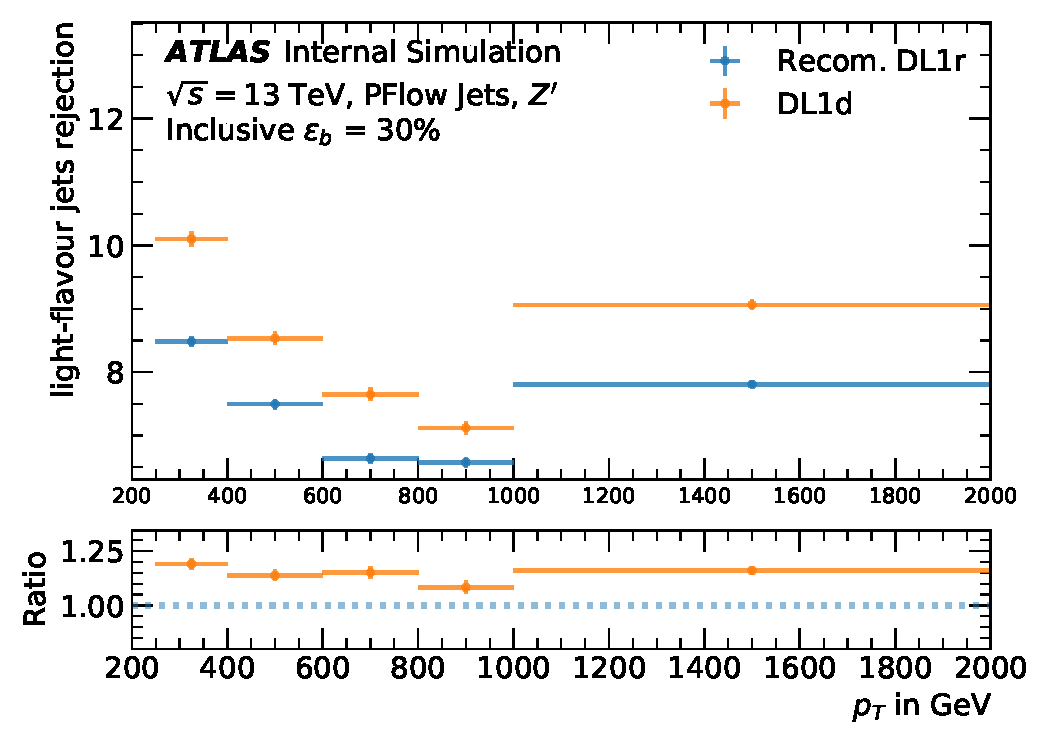
\includegraphics[scale=0.425]{Images//FTAG/Reprocessed/plotting_eff_vs_pt_c/pT_vs_beff_u_zp_299.pdf}
}
\caption{Background flavour rejections at a fixed $c$-tagging efficiency of 30\% (per region shown) for the various taggers. Top: $t\bar{t}$; bottom: $Z'$; left: $b$-rejection; right: light-rejection. For each plot, the bottom panel presents the ratio to the recommended \gls{dl1r}.}
\label{fig:ptDL1dz}
\end{figure}
\end{center}

In Figures \ref{fig:DL1dtt} and \ref{fig:DL1dz}, a new tagger currently in development is introduced: \gls{gn1} \cite{ATL-PHYS-PUB-2022-027}. This model is based on a graph neural network directly processing low-level inputs, thereby diverging from the traditional ATLAS flavour tagging philosophy of combining several low-level sub-taggers into a high-level one, such as in \gls{dl1d}. \gls{gn1} uses the information associated with charged tracks in a jet to directly output the flavour-tag probabilities, which are then combined into analogous discriminants to Equations \ref{bdisc} and \ref{cdisc}. Alongside predicting the flavour of the jet flavour, two auxiliary objectives are also optimised for the training: 
\begin{itemize}
\item the physics process that produced the different tracks and
\item grouping the tracks into vertices.
\end{itemize}
These complementary objectives improve performance and provide useful information on the content of the jets. Thanks to this guided training procedure, \gls{gn1} is able to compete favourably with the higher-level taggers presented so far, with on average a remarkable increase in the background flavour rejection for all tagging efficiencies. Another non-negligible advantage of the \gls{gn1} approach is the simplification of the structure, removing the need to maintain and retune several low-level algorithms. At the time of compiling the results, this tagger is still in development and is included solely to offer an exciting suggestion of the future performance of the tools deployed by the ATLAS flavour tagging group. 

\section{Conclusion}
This chapter introduces the novel tagger \gls{dl1d} to the set of flavour tagging tools available in ATLAS. Based on the \gls{dips} sub-tagger, \gls{dl1d} is found to have improved background rejections at a fixed working point for both $b$- and $c$-tagging. In parallel to the development of this new tagger, the preprocessing pipeline has been revamped and several changes to the input features list and model architecture were explored in order to deliver the best-performing tagger to the collaboration. 
\clearpage
